\documentclass{beamer}
\usepackage[utf8]{inputenc}
\usepackage{fontspec}
\usepackage{amsfonts,amsmath,amssymb}
\usepackage{url}
\usepackage{units}
\usepackage{xcolor}
\setmainfont{Liberation Serif}

\definecolor{drkgreen}{RGB}{59,107,0}
\newcommand{\pro}[1]{\textcolor{drkgreen}{#1}}
\newcommand{\con}[1]{\textcolor{red}{#1}}

\usetheme{Warsaw}
\useoutertheme{infolines}
\useinnertheme{rectangles}
\usecolortheme{beaver}
\setbeamerfont{title}{family=\rm}

\title[DAQ Update]{VFPIX Silicon Telescope \\ DAQ Board Update}
\author[C. Fangmeier]{Caleb Fangmeier}
\institute[UNL]{Univ.\ of Nebraska \-- Lincoln}
\date{September 28, 2015}

\begin{document}

\begin{frame}[plain]
  \titlepage
  \addtocounter{framenumber}{-1}
\end{frame}


\begin{frame}{Telescope Block Diagram}
  \centering
  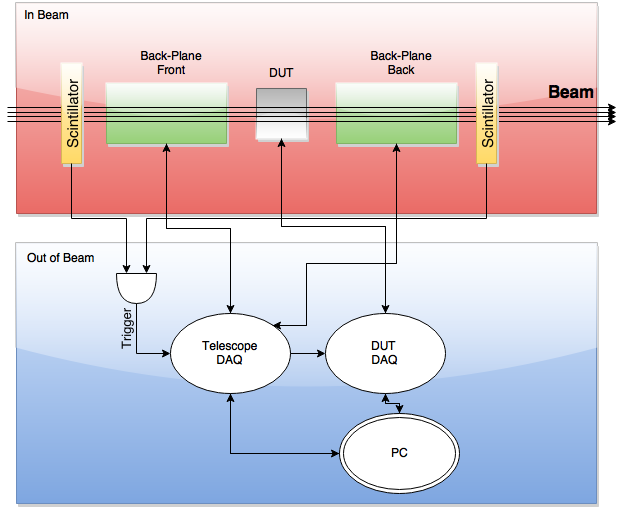
\includegraphics[height=0.9\textheight]{figures/Telescope_Hierarchy}
\end{frame}

\begin{frame}{Telescope Block Diagram}
  \centering
  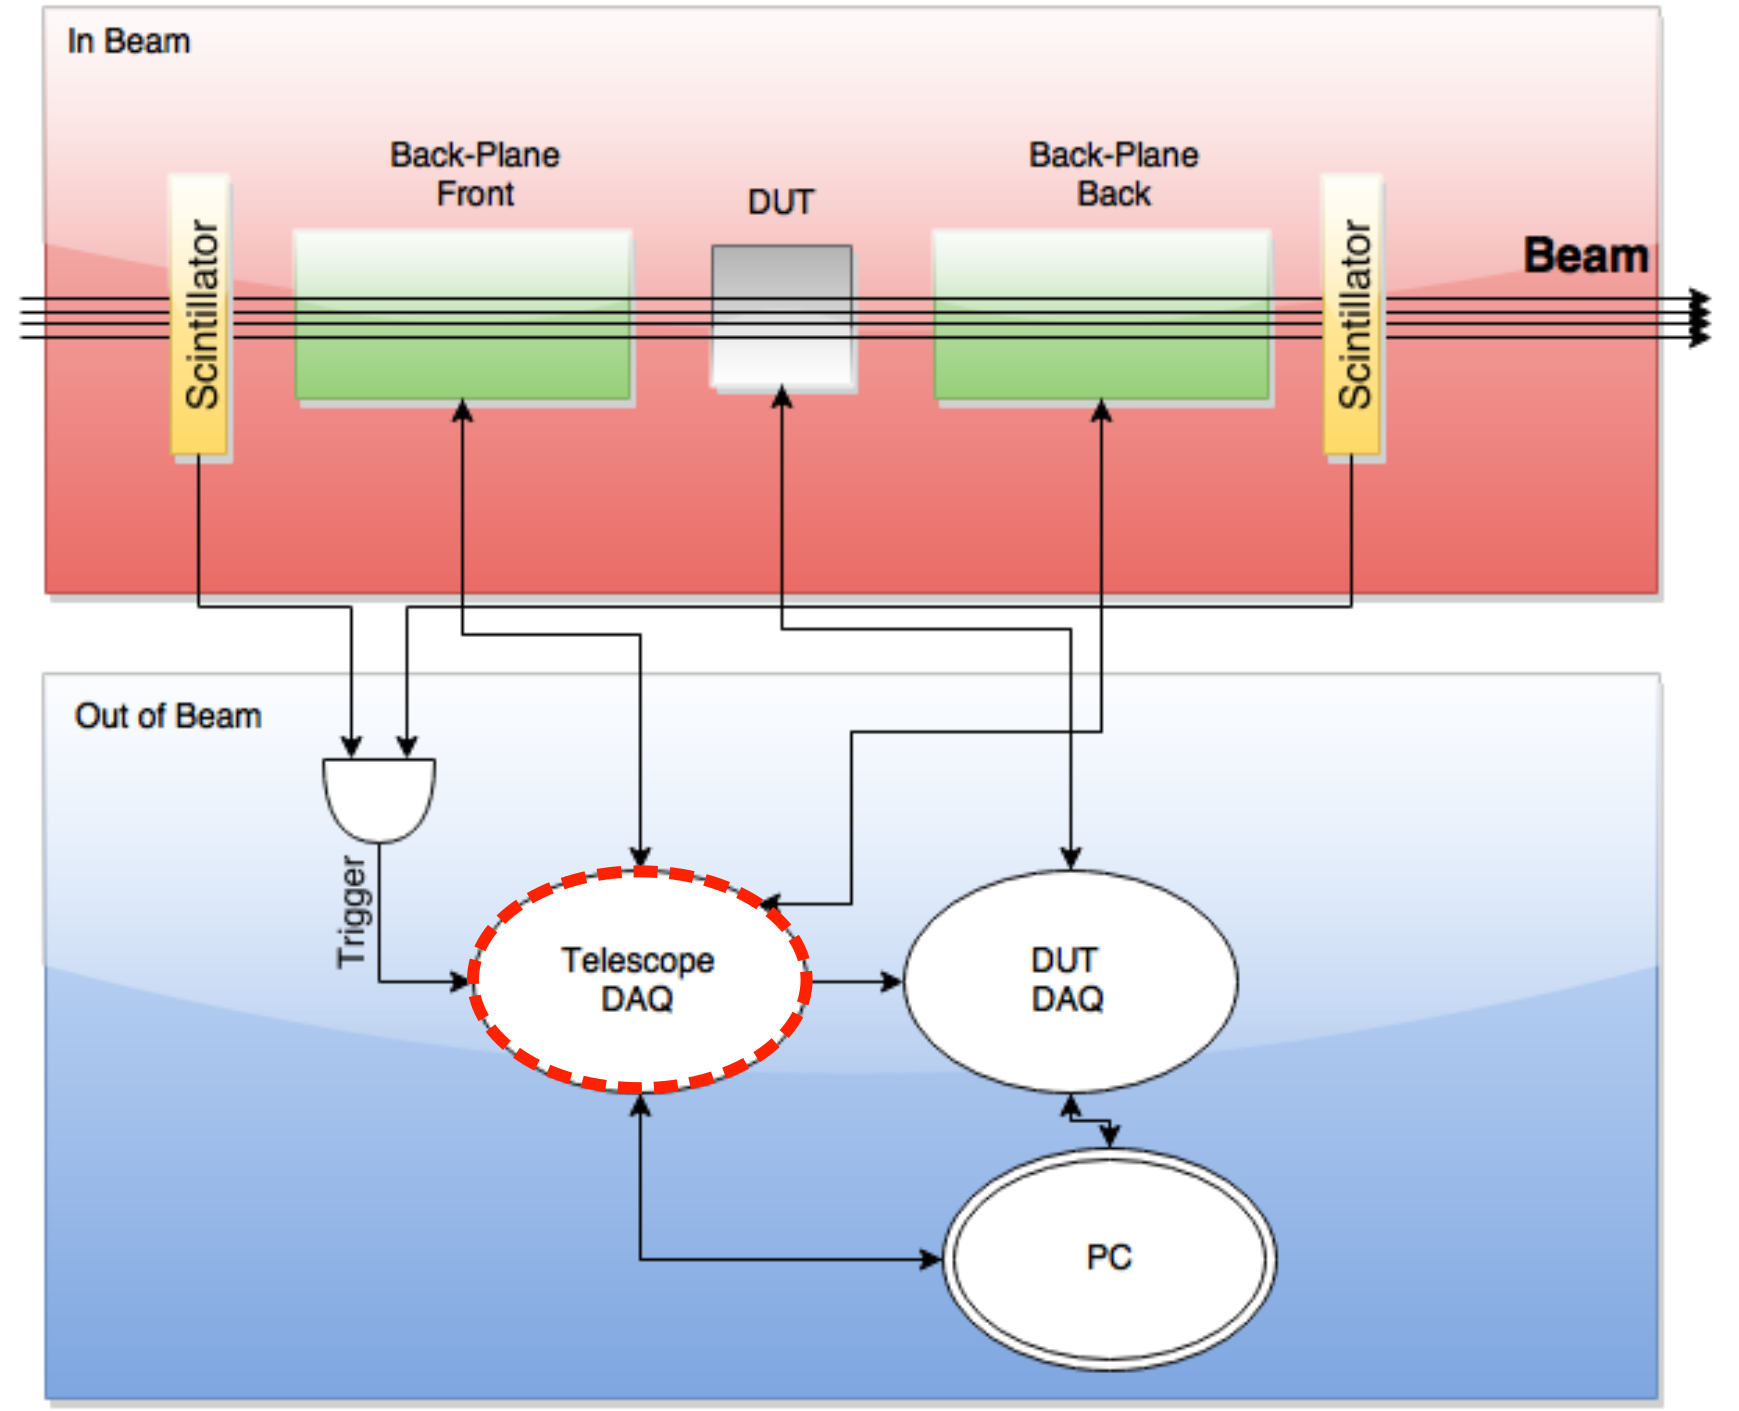
\includegraphics[height=0.9\textheight]{figures/Telescope_Hierarchy_Emph}
\end{frame}

\begin{frame}{Full DAQ - Front}
  \centering
  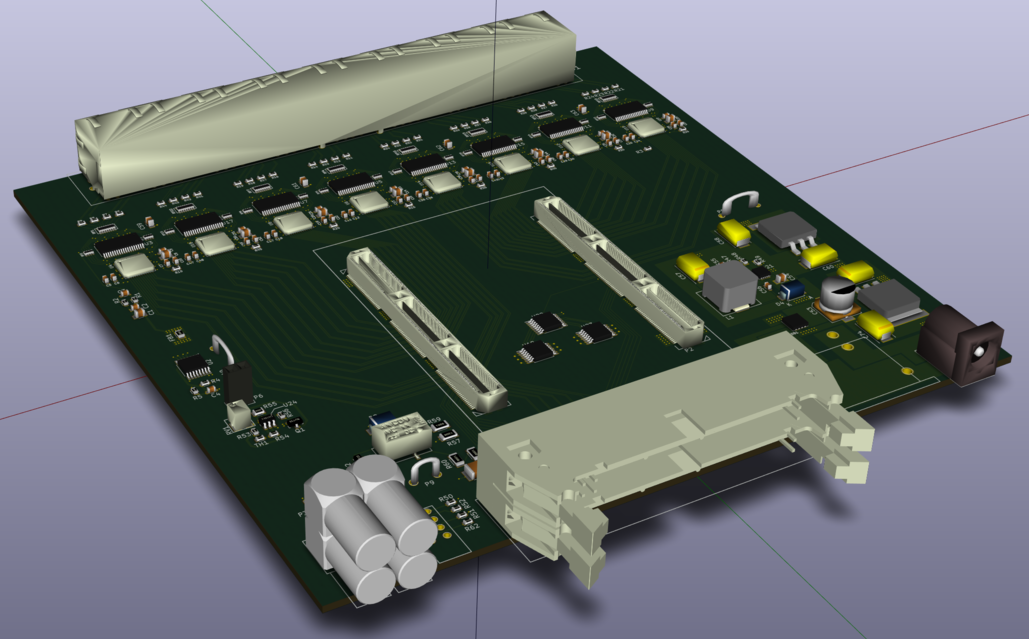
\includegraphics[width=0.95\textwidth]{figures/DAQCard2015_Full_Front_small}
\end{frame}

\begin{frame}{Full DAQ - Rear}
  \centering
  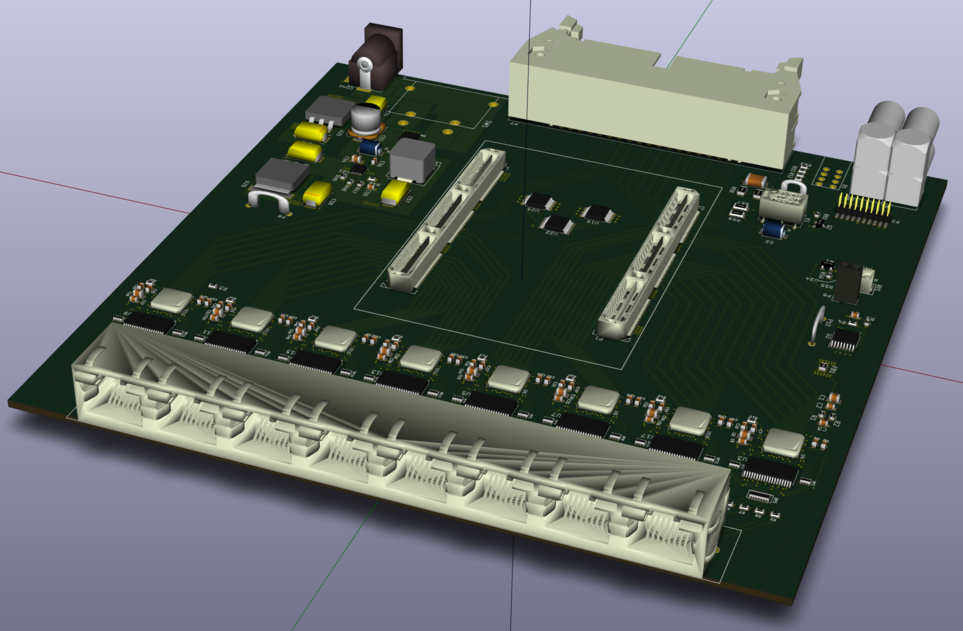
\includegraphics[width=0.95\textwidth]{figures/DAQCard2015_Full_Back_small}
\end{frame}

\begin{frame}{Single Input Channel}
  \centering
  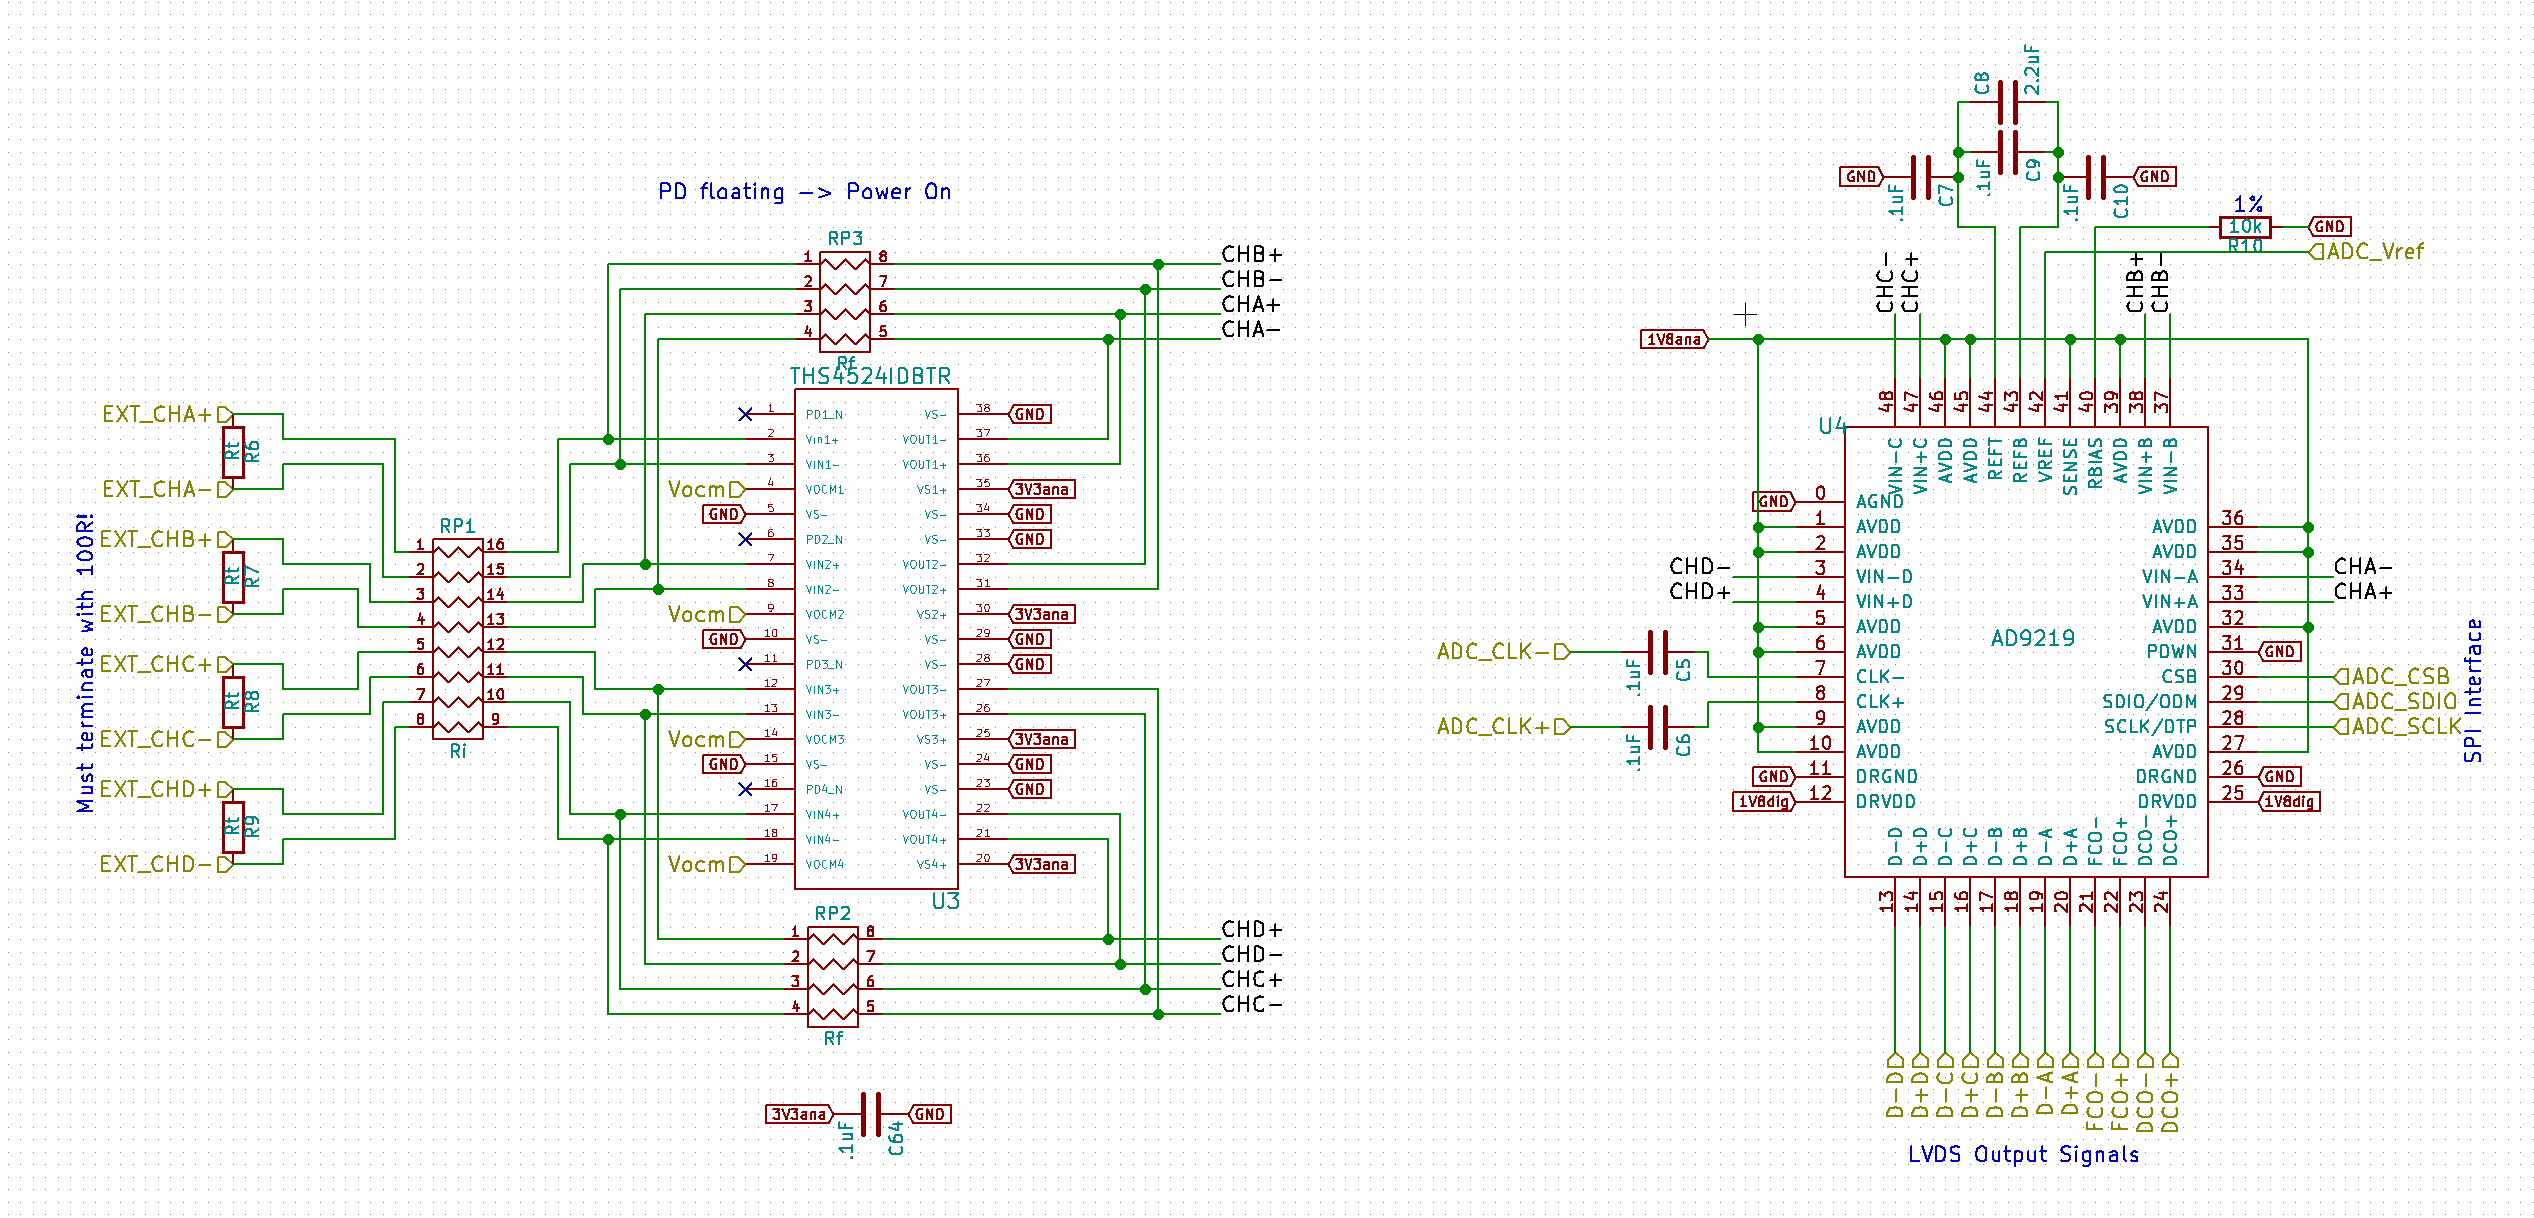
\includegraphics[width=\textwidth]{figures/Single_Channel_Schem}
\end{frame}

\begin{frame}{Single Input Channel}
  \centering
  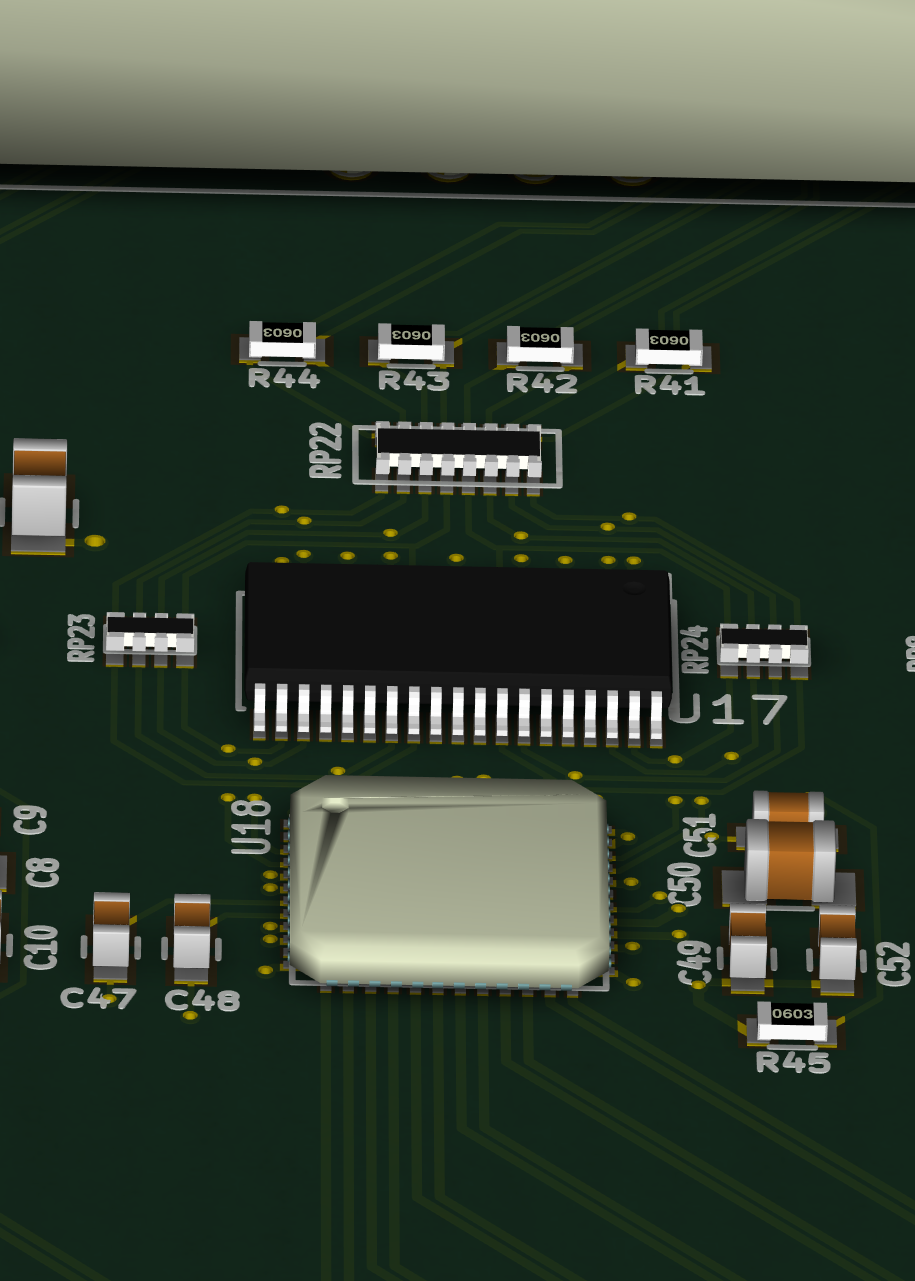
\includegraphics[height=\textheight]{figures/DAQCard2015_Single_Channel}
\end{frame}

\begin{frame}{Power Management}
  \centering
  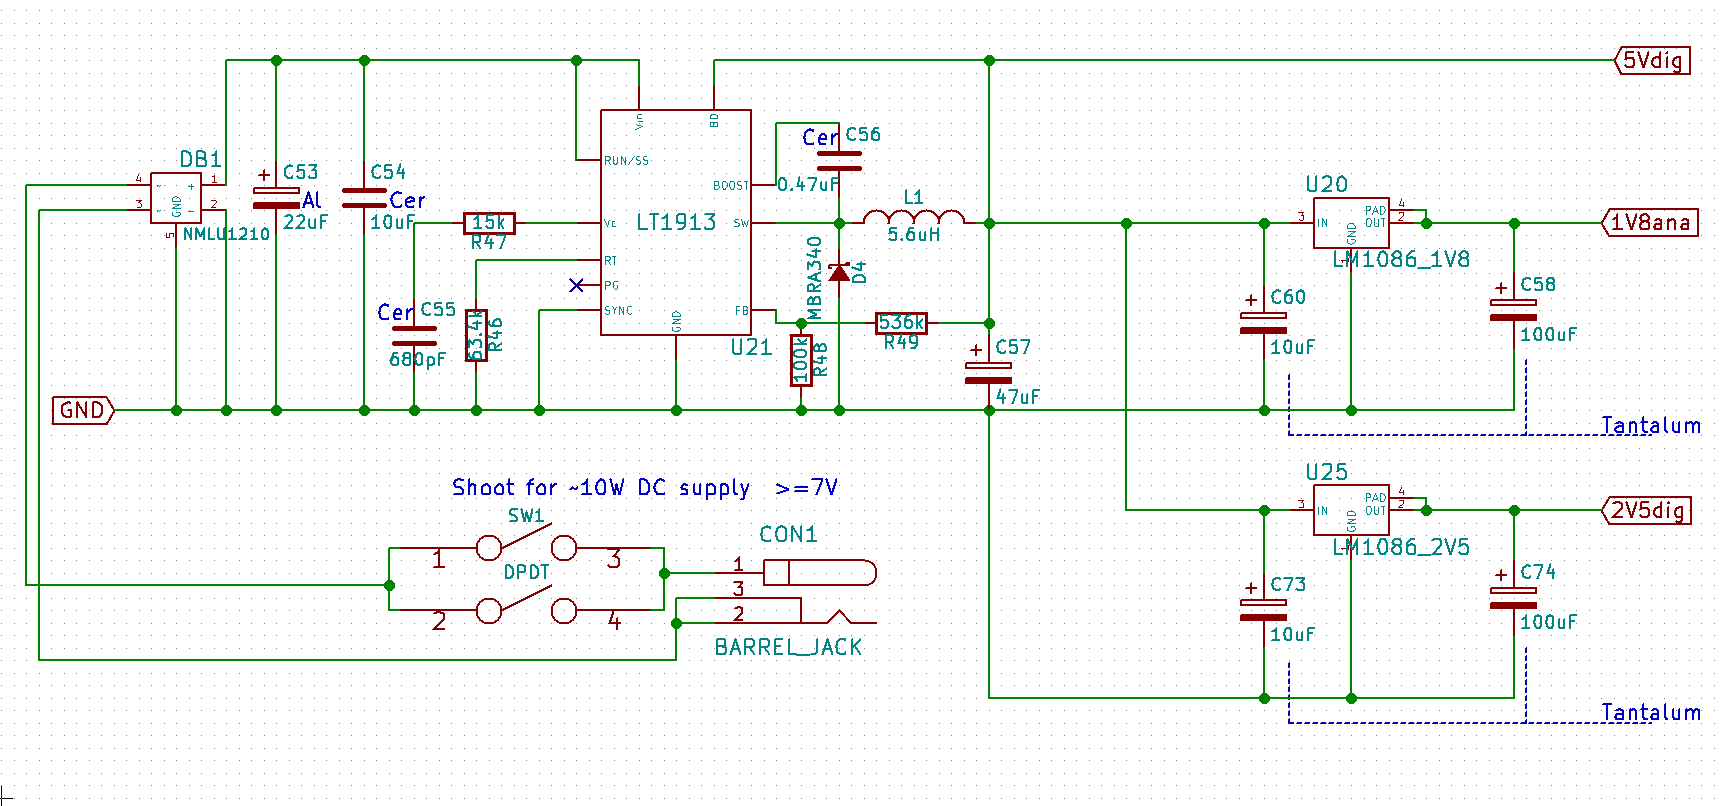
\includegraphics[width=\textwidth]{figures/Power_Schem}
\end{frame}

\begin{frame}{Power Management}
  \centering
  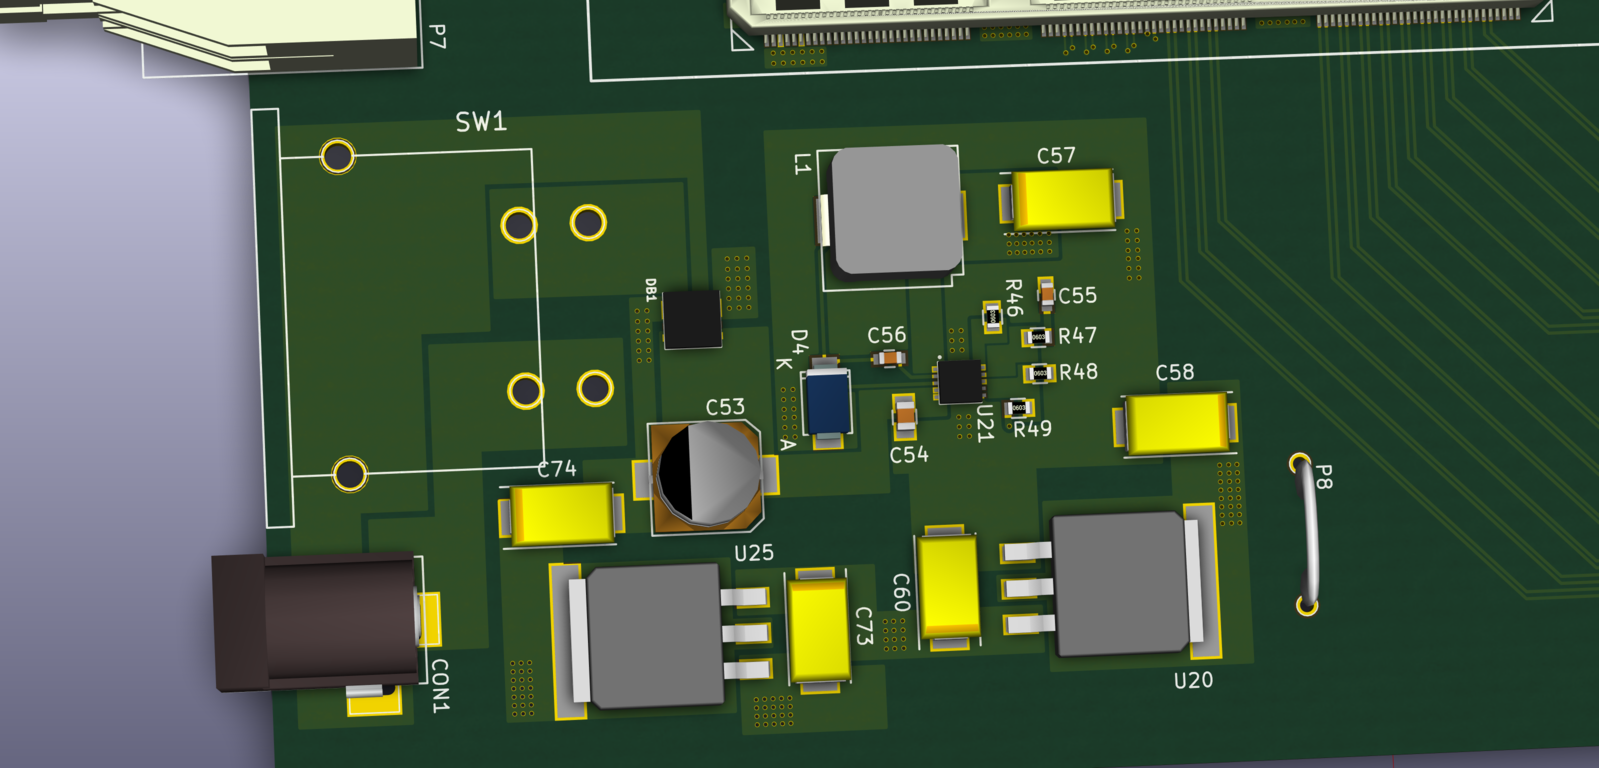
\includegraphics[width=0.95\textwidth]{figures/DAQCard2015_Power_small}
\end{frame}

\begin{frame}{Fan Control}
  \centering
  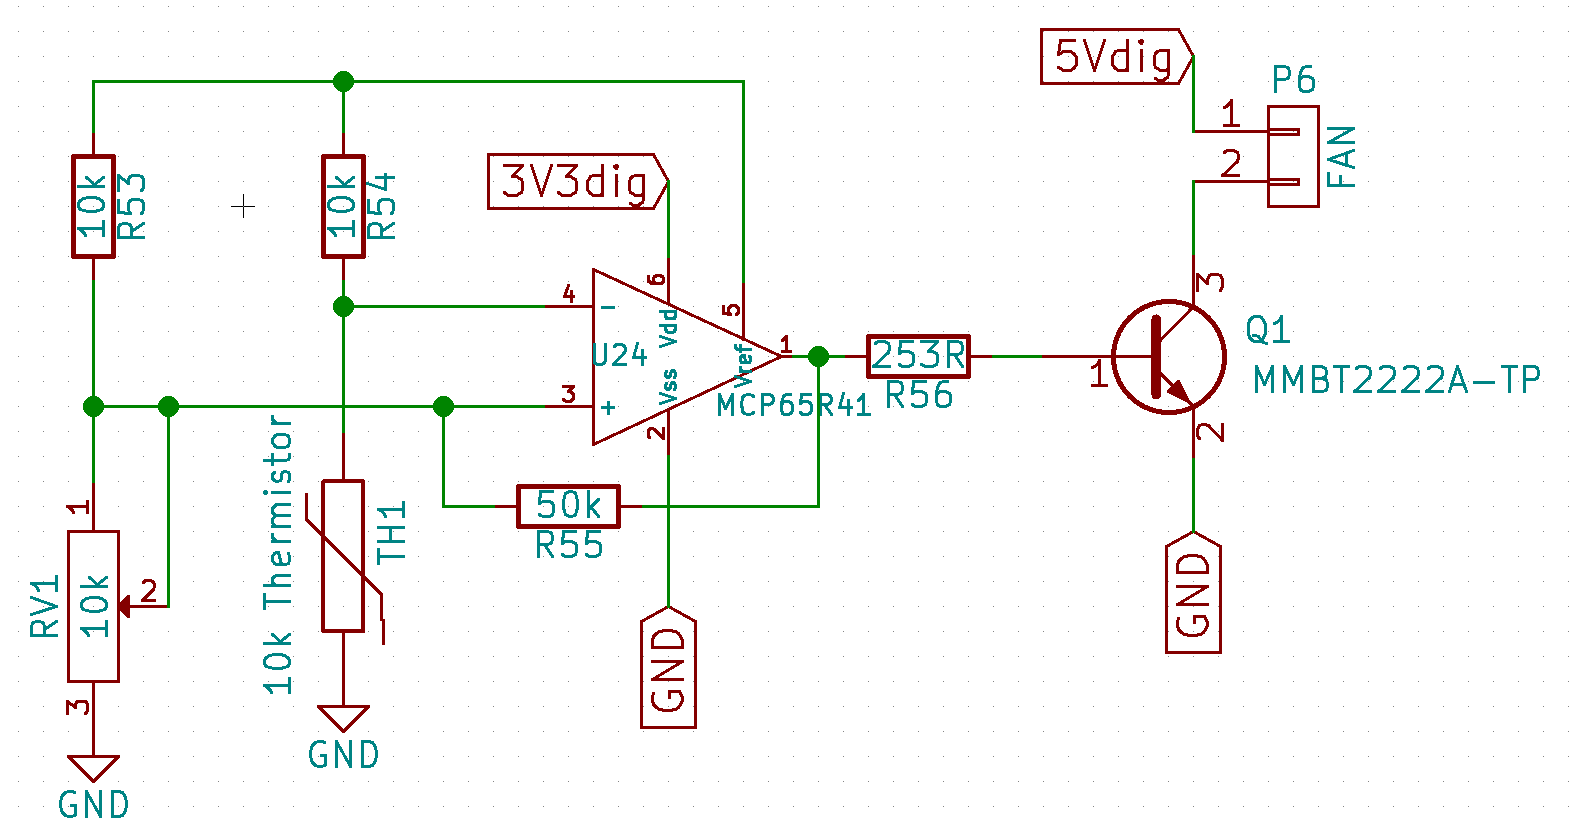
\includegraphics[width=\textwidth]{figures/Fan_Control_Schem}
\end{frame}

\begin{frame}{Fan Control}
  \centering
  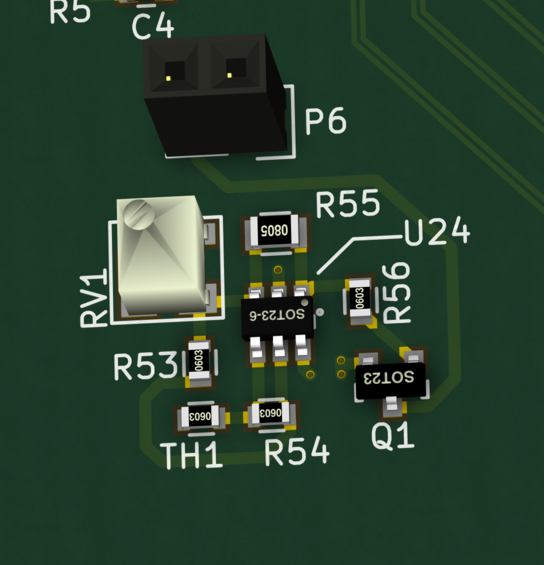
\includegraphics[height=\textheight]{figures/DAQCard2015_Fan_Control_small}
\end{frame}

\begin{frame}{APC128 Analog Voltage Supplies}
  \centering
  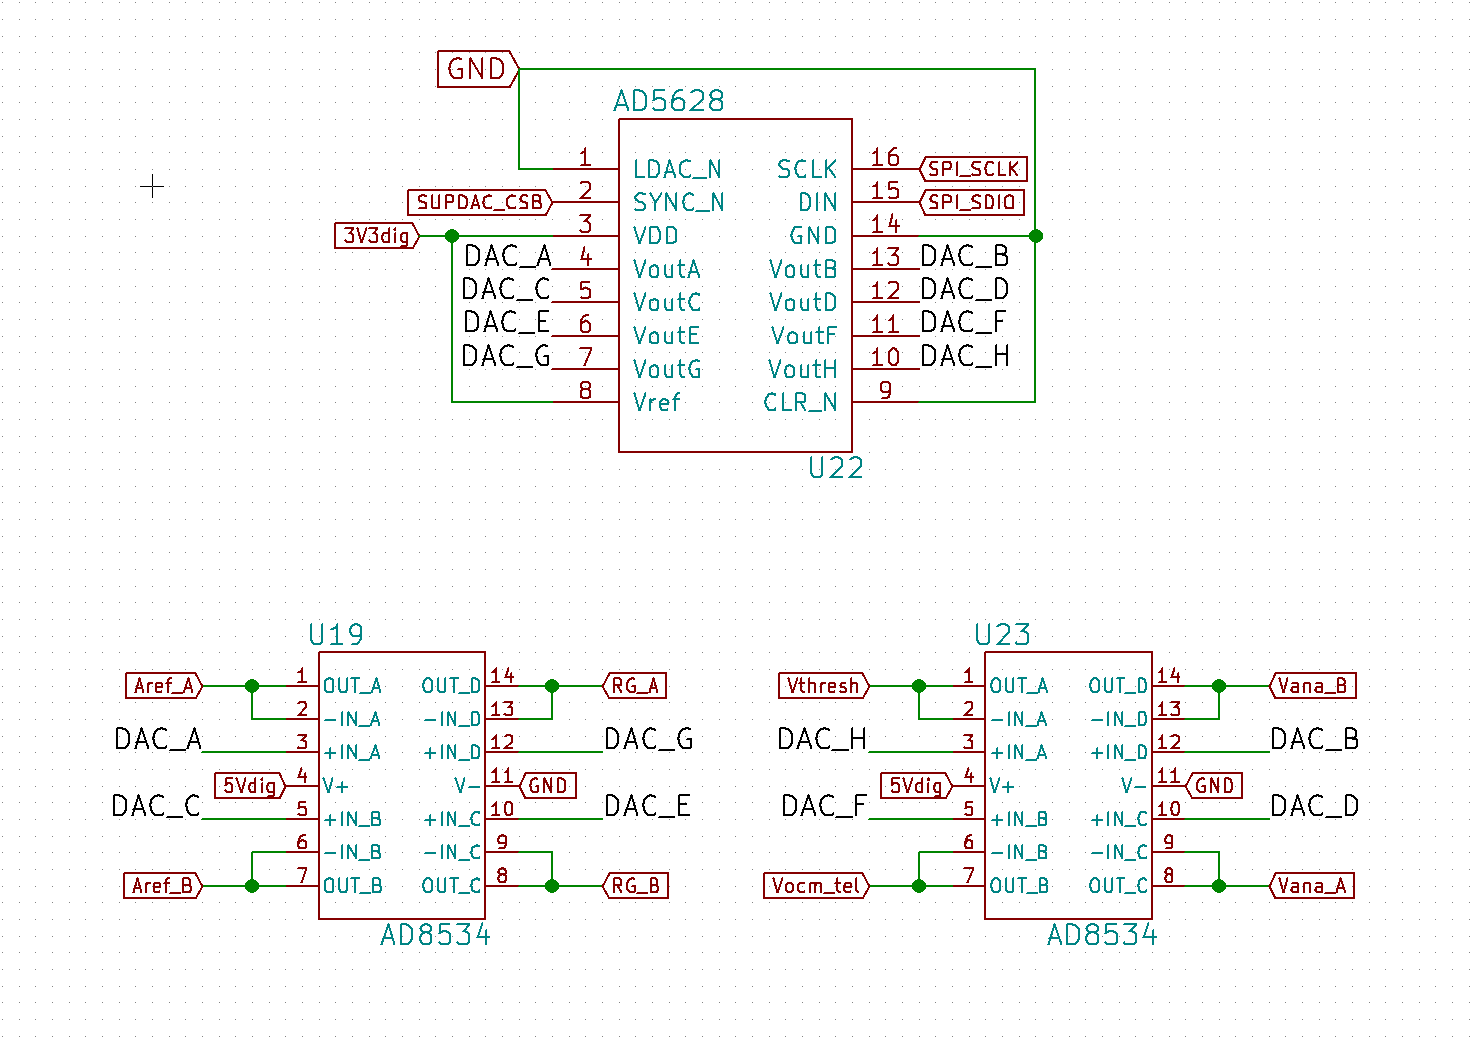
\includegraphics[width=\textwidth]{figures/Analog_Supply_Schem}
\end{frame}

\begin{frame}{APC128 Analog Voltage Supplies}
  \centering
  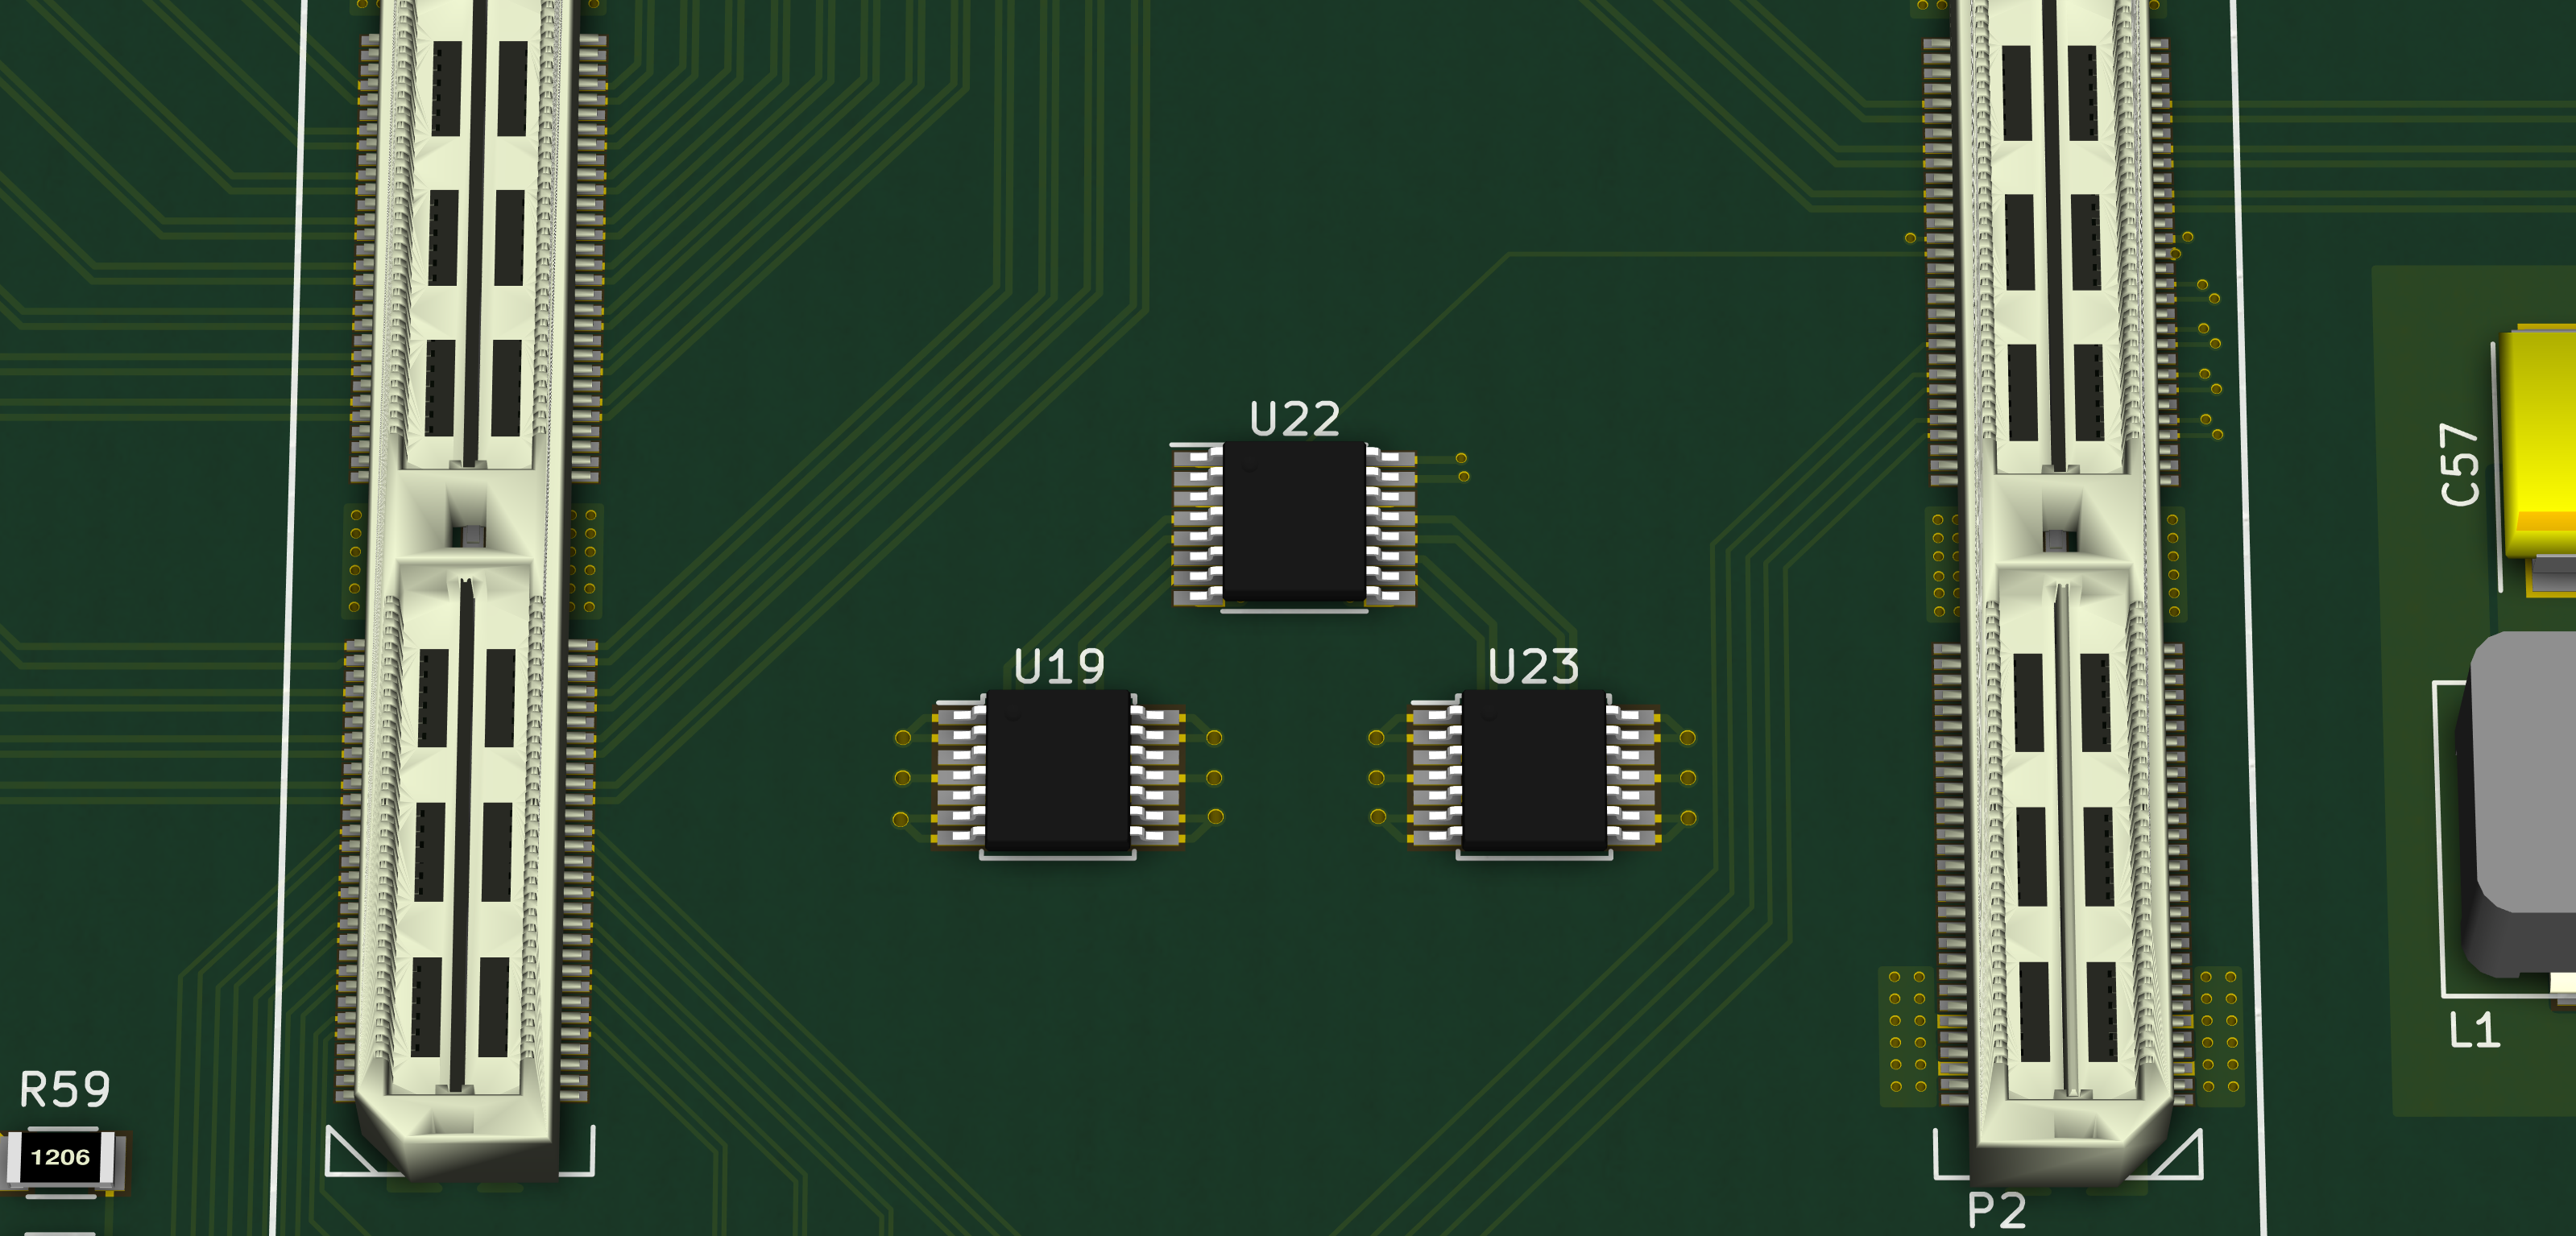
\includegraphics[width=\textwidth]{figures/DAQCard2015_Analog_Supply}
\end{frame}

\begin{frame}{Bias Voltage Control}
  \centering
  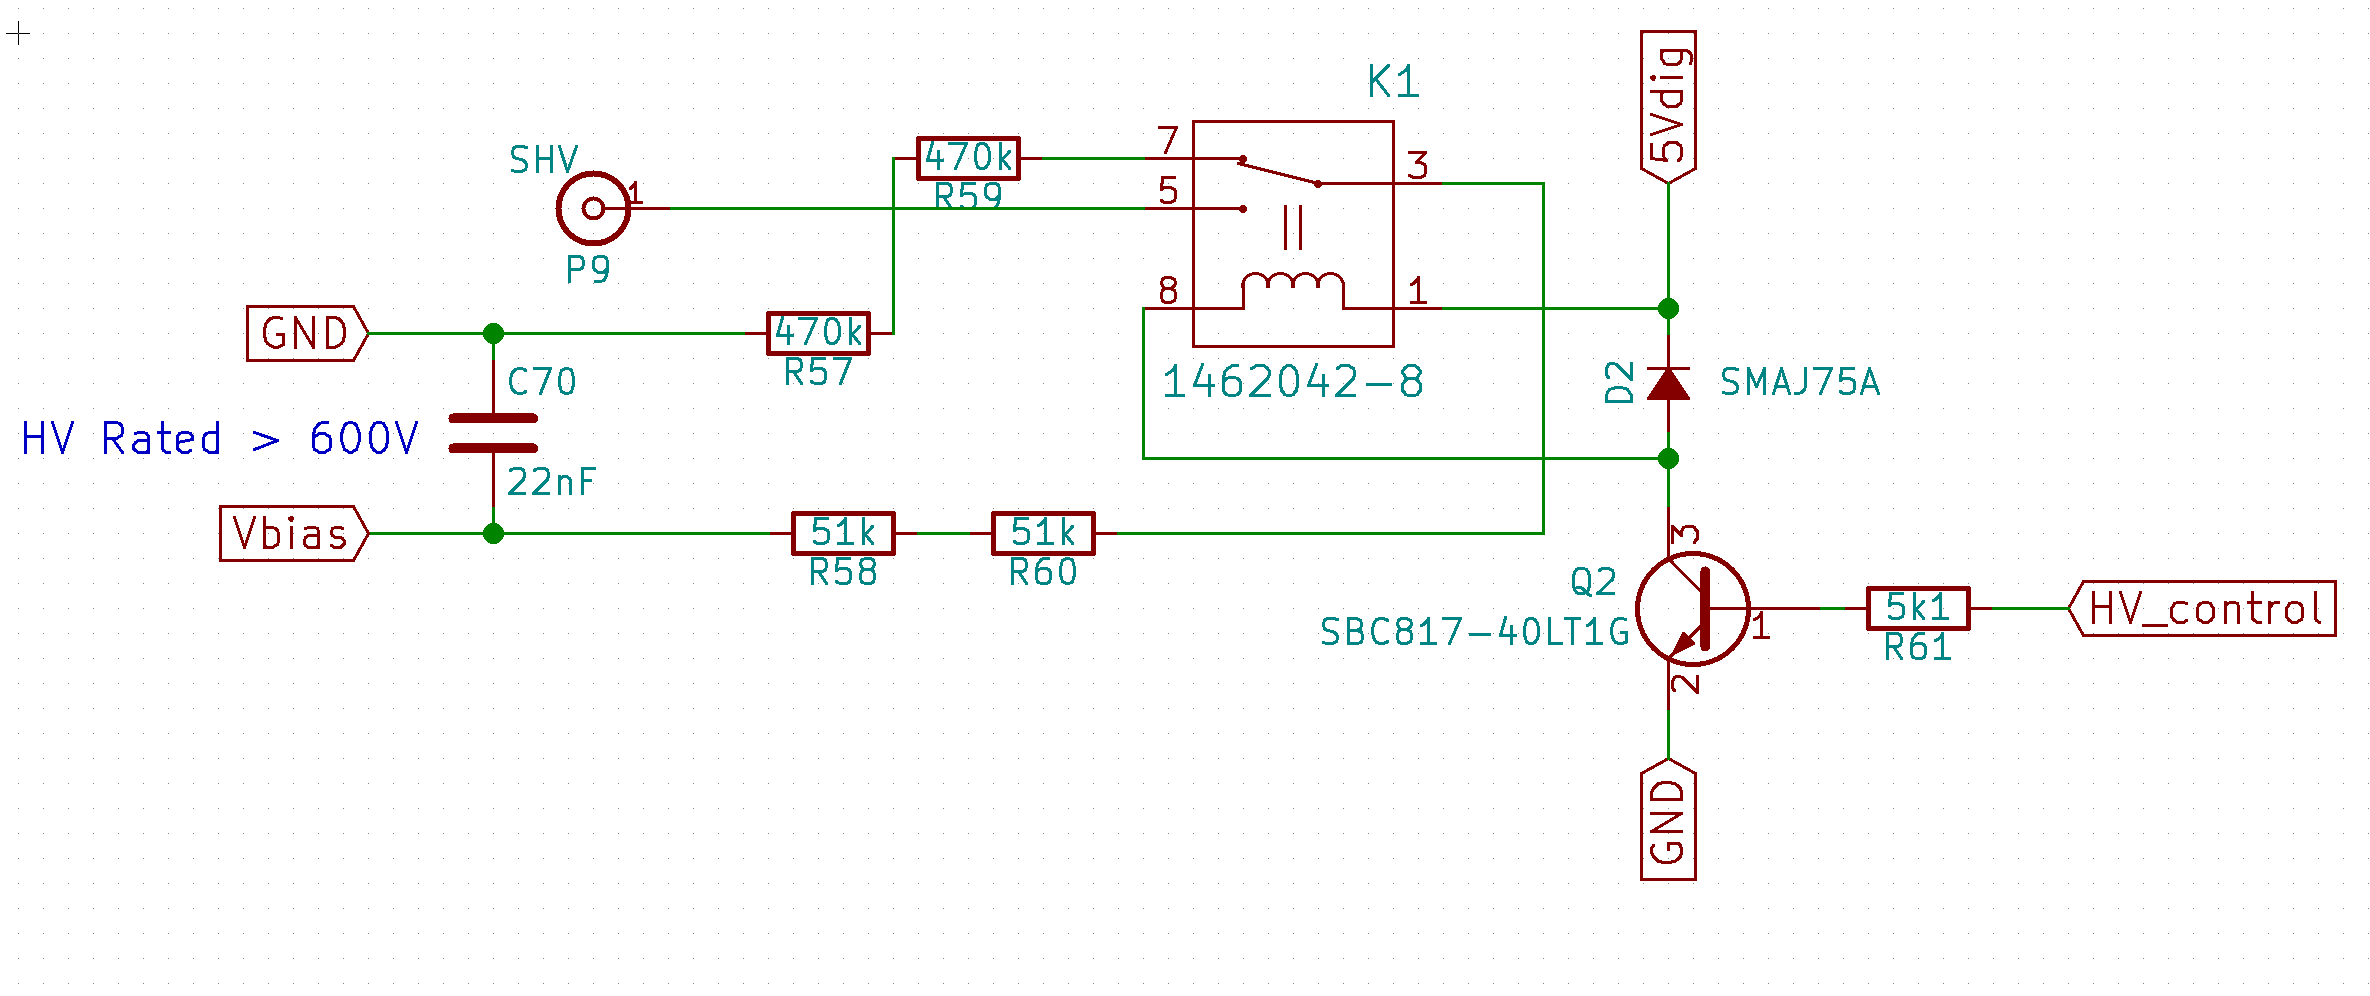
\includegraphics[width=\textwidth]{figures/HV_Schem}
\end{frame}

\begin{frame}{Bias Voltage Control}
  \centering
  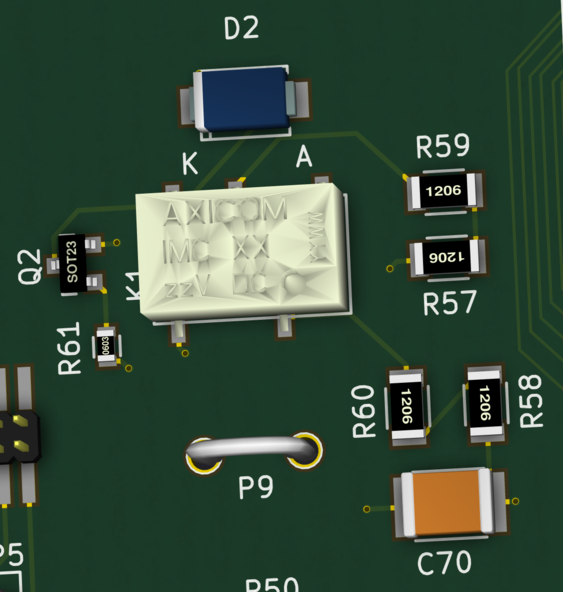
\includegraphics[height=\textheight]{figures/DAQCard2015_HV_small}
\end{frame}
\end{document}
